\AtBeginDocument{
  \hypersetup{
    pdftitle = {Cross-platform native GUIs},
    pdfauthor = {Zakariyya Mughal},
    pdfkeywords = {GUI, cross-platform, Perl}
  }
}

\title{Cross-platform native GUIs}
\providecommand{\subtitle}[1]{}
\subtitle{\{trade,pay\}offs, \{integra,distribu\}tion}
\author{Zakariyya Mughal}
\date[2021-06-10]{2021-06-10 \\[2ex]
{The Perl and Raku Conference (In the Cloud) 2021} \\[2ex]
\qrcode{https://github.com/zmughal-biblio/talk-tprc2021cic-cross-platform-native-guis-20210610}\\[1ex]
\btVFill
%
{\tiny\url{https://github.com/zmughal-biblio/talk-tprc2021cic-cross-platform-native-guis-20210610}}
}


\begin{document}
\frame{\titlepage}

\section{Motivation}

\begin{frame}
\protect\hypertarget{motivation}{}

\begin{longtable}[]{@{}cc@{}}
\toprule
	\begin{minipage}[t]{0.38\columnwidth}\centering
		\href{https://www.manning.com/books/operations-anti-patterns-devops-solutions}{Operations Anti-Patterns, DevOps Solutions}
		by Jeffery D. Smith\strut
	\end{minipage}
	&
	\begin{minipage}[t]{0.33\columnwidth}\centering
		\href{https://press.stripe.com/#working-in-public}{Working in Public}
		by Nadia Eghbal\strut
	\end{minipage}
	\tabularnewline
\midrule
\endhead

	\begin{minipage}[t]{0.38\columnwidth}\centering
		\begin{tikzpicture}
		  \node (book1) {
\includegraphics[height=3cm]{gfx/book-cover-OperationsAntiPatternsDevOpsSolutions.png}};
		  \node (author1) at (book1.south east) {
\includegraphics[height=1cm]{gfx/author-JeffreyDSmith.jpg}};
		\end{tikzpicture}
		\strut
	\end{minipage}
	&
	\begin{minipage}[t]{0.33\columnwidth}\centering
		\begin{tikzpicture}
		  \node (book2) {
\includegraphics[height=3cm]{gfx/book-cover-WorkingInPublic.png}};
		  \node (author2) at (book2.south east) {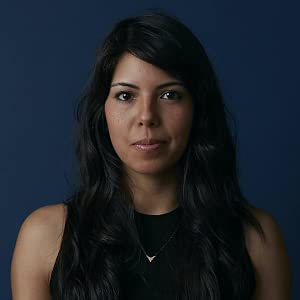
\includegraphics[height=1cm]{gfx/author-NadiaEghbal.jpg}};
		\end{tikzpicture}
		\strut
	\end{minipage}
	\tabularnewline
\bottomrule
\end{longtable}
	\note{Power law distribution in FOSS contributions}
\end{frame}

\section{The competition}

\subsection{Put on developer hat}

\begin{frame}{Web applications are great} % Compare with web app + pros of using web app (for developers)
\protect\hypertarget{the-competition}{}

\note{
I am now going to be slightly polemical to persuade,
    but don't worry, I'll get to the technical parts quickly.
}

\begin{itemize}
\tightlist
\item
  $\underset{\text{for developers}}{\text{Easy deployment}}$ →
     $\underset{\text{for users}}{\text{Easy update}}$
  \note{ No fiddling with installers, no ABI compatibility issues.
	If this is your top priority, use a web application. }
\item
  Flexible declarative languages for \emph{separation of content and
  presentation}.

  \begin{itemize}
  \tightlist
  \item
    HTML, CSS, MathML, SVG
    \note{ These are useful outside the context of web applications. }
  \end{itemize}
\end{itemize}

\note{
Note on recursive use of web standards:

You can embed an \texttt{iframe} and other HTML inside of SVG using \texttt{foreignObject}.
But you can not easily render HTML to an HTML Canvas or WebGL — this is not
allowed because it can be a \href{https://stackoverflow.com/questions/6335383/render-html-in-canvas-webgl}{security risk}.
}

\end{frame}

\begin{frame}{But there are drawbacks} % Cons of using web app (for developers)

\begin{itemize}[<+->]
\tightlist
\item
  Web browsers are a sandbox for a reason.
  \note{ They are designed for dealing with the web and all the security
      concerns behind that. But sometimes one persons ``security concerns'' is another
          person's ``yes, I really meant to do that Clippy''. }
\item
  Platform + browser combination bugs.
  \note{ Go look on the bug trackers for browsers. }
\item
  Polyfills/shims are\ldots{} \alert<.>{dirty}
\end{itemize}

\end{frame}

\begin{frame}{I want to do X, Y, \& Z}
\begin{itemize}[<+->]
\tightlist
\item
  Lots of useful native code already exists that would need to
  reimplemented.

  \begin{itemize}[<+->]
  \tightlist
  \item
    Yes, we have WebAssembly. And tooling like Emscripten.
  \item
    But package management is incomplete. And packages are not
    well-tested.
  \end{itemize}

\item
  Accessing that code through a client-server architecture adds overhead
  for some applications.
\end{itemize}

\note{
For example, packages could have duplicate versions of libpng inside of them.
Not to mention the bandwidth problems if everybody distributes packages like this.

There should be a lot of appreciation for system package maintainers for making
sure that dependencies between packages work with all the downstream packages.
}
\end{frame}

\begin{frame}{Computing APIs} % Web APIs compared with native APIs

\newcommand{\techyear}[2]{\(\underset{\text{\tiny{}#2}}{\text{#1}}\)}
\begin{longtable}[]{@{}ll@{}}
\toprule
Native & Web browser\tabularnewline
\midrule
\endhead
\techyear{OpenGL}{1992}, \techyear{OpenCL}{2009}, \techyear{Vulkan}{2016} & \techyear{WebGL}{2011}, \techyear{\sout{WebCL}}{2014}, \techyear{WebGPU}{upcoming}\tabularnewline
\techyear{OS threads}{1960s} & \techyear{Web Workers}{2008--2010}, \techyear{Worklet}{2015--}\tabularnewline
daemon process & \techyear{Service Workers}{2014}\tabularnewline
\techyear{(TCP) socket}{1970--1980} & \techyear{WebSocket}{2011}\tabularnewline
key-value store library & \techyear{Web storage}{2009}, \techyear{\sout{WebSQL}}{2010}, \techyear{IndexedDB}{2015}\tabularnewline
machine data types & \techyear{typed arrays}{2011}\tabularnewline
\bottomrule
\end{longtable}

\note{
KV store, e.g., SQLite (2000) (sql.js!), LevelDB (2011)

Initially browsers had very little access to computing resources, but
now we have these (see table).


Other APIs at \url{https://developer.mozilla.org/en-US/docs/Web/API}, e.g., Web Speech API, Gamepad API.

But this is always going to be delayed from where computer hardware is. Feature
support has to filter through the OS, compiler/user-space library, browser/standards
unless hardware is designed specifically for the browser.

Creating standards is a lot of work. I'm certain that code to give access to
native features can be done by simply binding to them (using IDL), but thinking
about making this in a way so that most platforms can implement a common subset
of that feature requires a lot of effort.
}

\end{frame}

\begin{frame}{Fusion?} % How to access more native APIs while still using web technologies

\begin{itemize}[<+->]
\tightlist
\item \textbf{Problem}
	Limited control over memory, storage, battery, and other
	resources.
	\note{ How resources are managed is left up to the browser implementation. }
\item \textbf{Solution}
	Embed a specific browser to provide a webview (\href{https://www.electronjs.org/}{Electron}, \href{https://nwjs.io/}{NW.js},
	\href{https://bitbucket.org/chromiumembedded/cef}{Chromium Embedded Framework}, \href{https://cordova.apache.org/}{Apache Cordova}).
\item
  Gives a lot of control over how resources are passed into the
  webview part of the application, e.g., through custom scheme handlers.
\end{itemize}

\note{
Much better than requiring a browser extension for using a web application.

Since all of these are based on Chromium, they can all be tested and controlled using the WebDriver protocol.

But certain platform + browser combination bugs will remain.
}

\end{frame}

\subsection{Put on user hat}
\begin{frame}{User data goes\ldots{} somewhere} % Cons of using web apps (for users)

Underappreciated values

\begin{itemize}[<+->]
\tightlist
\item
Privacy
\item
Data interoperability
\item
Future-proof (backups, format shifting)
\note{ During the course of gathering resources, several of my bookmarks
	  are no longer available on the web or Internet Archive
	  because they used JavaScript to retrieve their content.

Web apps make the web less machine-readable.}
\item Integration with the desktop
\end{itemize}

\end{frame}
\begin{frame}{User data goes\ldots{} somewhere} % Cons of using web apps (for users)

\uncover<+->{
Data interoperability can provide \emph{separation of data and
application}.
}

\uncover<+->{
Possible solution in \href{https://solidproject.org/}{Solid}.

\begin{center}
	\begin{tikzpicture}
	  \node (solid) {
\includegraphics[height=5cm]{gfx/Solid-Protocol.png}};
	\end{tikzpicture}
\end{center}
}

\end{frame}

\begin{frame}{The Lost City of Interaction Design} % More cons of using web apps (for users)

Integration between applications is limited or sometimes broken:

  \begin{itemize}[<.->]
  \tightlist
  \item
    Clipboard
    \note{ I saw a bug about copying SVG into the clipboard and different browsers implement this differently. }
  \item
    Drag-and-drop
  \end{itemize}

\end{frame}
\begin{frame}{The Lost City of Interaction Design} % More cons of using web apps (for users)

Widgets are often very non-desktop like:

  \begin{itemize}[<+->]
  \tightlist
  \item
    Frameworks exist, e.g.,
    \href{https://qooxdoo.org/}{qooxdoo}
    %\footnote<+->{Check out \href{https://metacpan.org/release/CallBackery}{CallBackery} on CPAN.}
  \item
    Not every widget supports:

    \begin{itemize}[<.->]
    \tightlist
    \item
      Jumping to items / incremental search
    \item
      Multi-level undo
    \item
      Binding all keyboard shortcuts
    \end{itemize}
  \end{itemize}

\end{frame}

\subsection{Put on carbon-based lifeform hat}
\begin{frame} % Human factors

\begin{columns}
  \begin{column}{0.48\textwidth}
	\begin{itemize}
	\tightlist
	\item
	  Visual system was made for object recognition, not reading.
	  \note{ Terminal CLIs and TUIs are not enough. }
	\item
	  Latency:\\
			\begin{center}
			input → render
			\end{center}
		\\
		feedback loop
	\end{itemize}
  \end{column}
  \begin{column}{0.48\textwidth}
	\begin{longtable}[]{@{}c@{}}
	\toprule
		\begin{minipage}[t]{0.80\columnwidth}\centering
			\href{https://dl.acm.org/doi/book/10.5555/333103}{The Humane Interface} by Jef Raskin
		\end{minipage}
		\tabularnewline
	\midrule
	\endhead
		\begin{minipage}[t]{0.80\columnwidth}\centering
			\begin{tikzpicture}
			  \node (book4) {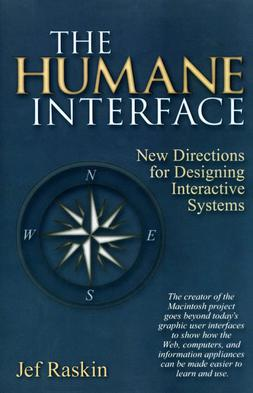
\includegraphics[height=3cm]{gfx/book-cover-TheHumaneInterface.jpg}};
			  \node (author4) at (book4.south east) {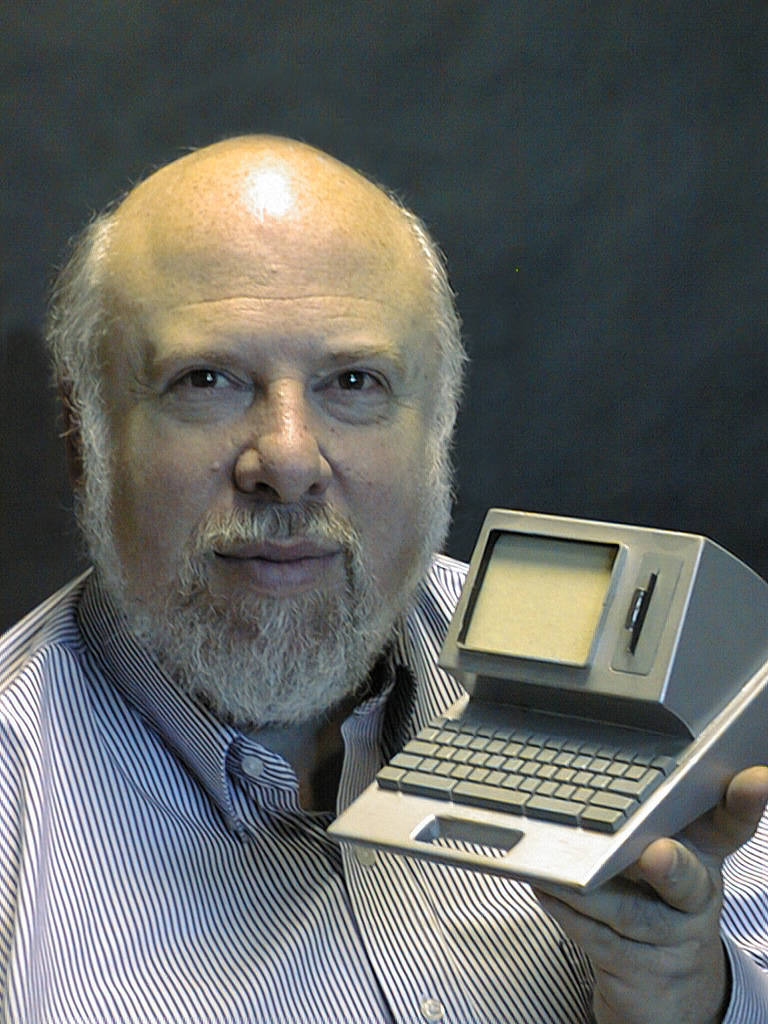
\includegraphics[height=1cm]{gfx/author-JefRaskin.png}};
			\end{tikzpicture}
			\strut
		\end{minipage}
		\tabularnewline
	\bottomrule
	\end{longtable}
  \end{column}

\end{columns}


\end{frame}

\subsection{Hardware}
\begin{frame}
	% e-ink reader
	% tablet
	% OLPC XO-1
	%  - spotify running under wine
	%  - swapping to SD card, SD card's have limited write cycles
	\usetikzlibrary{positioning}
	\begin{minipage}[t]{0.80\columnwidth}\centering
		\begin{tikzpicture}
			\begin{scope}[node distance=0.5cm]
				\node (center) at (0,0);
				\node[above = of center] (kindle) {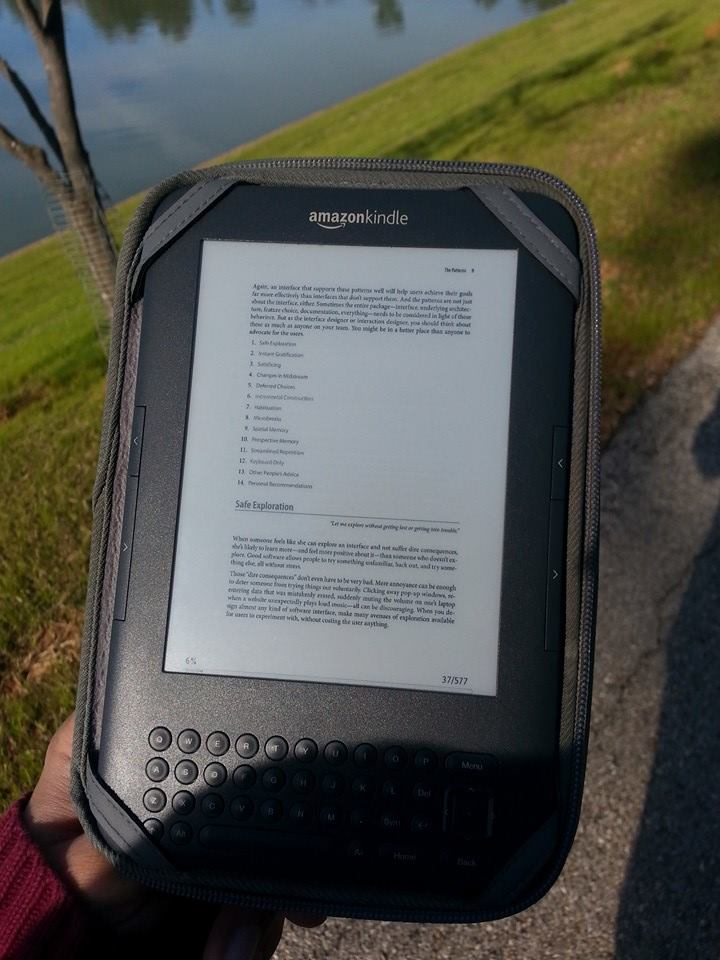
\includegraphics[height=3cm]{gfx/kindle-in-action.jpg}};
				\node[below right = of center] (xo1) {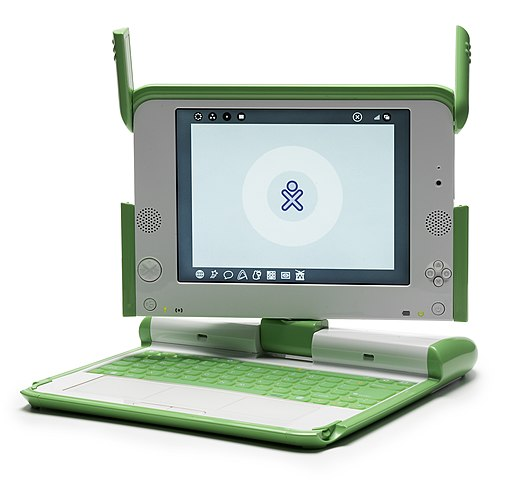
\includegraphics[height=3cm]{gfx/520px-XO-Beta1-mikemcgregor-2.jpg}};
				\node[below left = of center] (tablet) {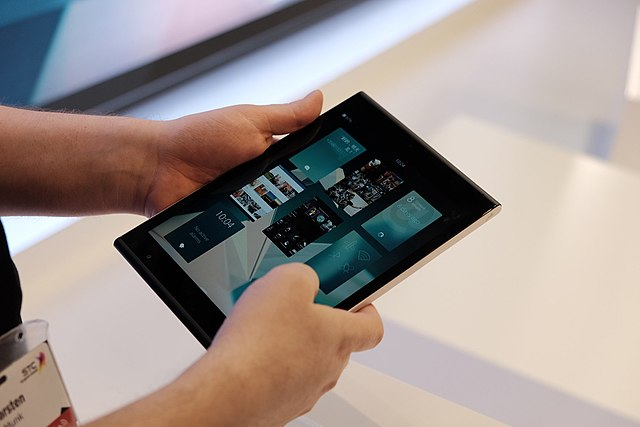
\includegraphics[height=3cm]{gfx/640px-Jolla_Sailfish_tablet_-_MWC_2015.jpg}};
			\end{scope}
		\end{tikzpicture}
		\strut
	\end{minipage}
\end{frame}

\section{Intermission}

\begin{frame}
	\paragraph{\emph{C shanty}}
	\begin{description}
		\item[]<+-> There once was a lib written in C \\
			Installing it was not easy
		\item[]<+-> Tried t'build on Win and go \\
			But linker failed, Bill said no
		\item[]<+-> Soon may the QA come \\
			But not until all checks are done
		\item[]<+-> The OS does segfault throw \\
			The buffer did overflow
	\end{description}
\note{ Is this what it means to ship it using Docker?  }
\end{frame}

\section{The technical part}
\begin{frame}{Solutions on CPAN \emph{today}}
\protect\hypertarget{gui-toolkits-on-cpan}{}

Cross-platform:

\begin{itemize}
\tightlist
\item
  \href{https://metacpan.org/pod/IUP}{IUP}
\item
  \href{https://metacpan.org/pod/Prima}{Prima}
\item
  \href{https://metacpan.org/pod/Fl}{Fl}
\item
  \href{https://metacpan.org/pod/Tk}{Tk}
\item
  \href{https://metacpan.org/pod/Tkx}{Tkx}
\item
  \href{https://metacpan.org/pod/Wx}{Wx}
\item
  \href{https://metacpan.org/pod/Gtk3}{Gtk3}
\end{itemize}

Other:

\begin{itemize}
\tightlist
\item
  \href{https://metacpan.org/pod/Win32::GUI}{Win32::GUI} (non-cross-platform),
  \href{https://metacpan.org/pod/Gtk2}{Gtk2} (old)
  \note{
  \href{https://gitlab.com/Kerenoc/GCstar}{GCstar} - collections manager (port to Gtk3 done)

  \href{https://github.com/shutter-project/shutter}{Shutter} - screenshot application

  \href{https://github.com/shawnlaffan/biodiverse}{Biodiverse} - spatial analysis tool (for understanding climate impacts)
  }
\end{itemize}

\end{frame}

\begin{frame}[fragile]{Gtk3}
	\begin{itemize}[<+->]
		\item Cross-platform
		\item Many language bindings provided through GObject Introspection.
		\item Glade interface builder
		\item \href{https://developer.gnome.org/gtk3/stable/gtk-running.html}{Interactive debugger}
{
%\setbeamercolor{block body}{bg=black, fg=white}
\setbeamercolor{block body}{bg=black}
\begin{block}{}
\begin{lstlisting}[language=sh,xleftmargin=10pt]
export GTK_DEBUG='interactive'
my-gtk-application
\end{lstlisting}
\end{block}
}
	\end{itemize}
\end{frame}

\begin{frame}{Gtk3 on *}
\begin{center}
\qrcode{https://github.com/orbital-transfer-example/perl-gtk3-starter-basic}

\url{https://github.com/orbital-transfer-example/perl-gtk3-starter-basic}
\end{center}
\end{frame}

\begin{frame}[fragile]{Gtk3 on Linux}
	\begin{itemize}[<+->]
		\item Use system package manager for native packages
		\item ``It just works.'' \uncover<+->{ --- me (ca. just now) }
		\item Docker: some tools don't like being run as root
	\end{itemize}
	\note{
		Use own Perl during development.

		Docker, no root (Anki --- Qt Web Engine, CEF ; both Chromium based)
	}
\end{frame}

\begin{frame}[fragile]{Gtk3 on macOS}
	\begin{itemize}[<+->]
		\item macOS has several package managers: tested with \href{https://brew.sh/}{Homebrew}
		\item Do not use system Perl (good advice for any platform)
		\item Architecture: \texttt{x86\_64}, will need testing on \texttt{arm64}: \url{https://doesitarm.com/}
	\end{itemize}
	\note{
		System Perl would list multiple architectures in
		\texttt{ccflags} which would break compilation of \texttt{Glib.pm} (see
		\texttt{ARCHFLAGS} environment variable and how it relates to universal binaries).

		See discussion at \url{https://mail.gnome.org/archives/gtk-perl-list/2016-October/msg00004.html}
		and \url{https://docs.brew.sh/Gems,-Eggs-and-Perl-Modules#avoiding-sudo-altogether-for-perl}.
	}
\end{frame}

\begin{frame}[fragile]{Gtk3 on MSWin32}
	\begin{itemize}[<+->]
		\item Use MSYS2.
		\item \texttt{ExtUtils::MakeMaker} hacks
		\item \href{https://docs.microsoft.com/en-us/windows/win32/fileio/maximum-file-path-limitation}{\texttt{\#define MAX\_PATH 260}}
		\item Disable layered windows
{
\setbeamercolor{block body}{bg=black}
\begin{block}{}
\begin{lstlisting}[language=Perl,xleftmargin=10pt]
BEGIN {
  if( $^O eq 'MSWin32' ) {
    $ENV{GDK_WIN32_LAYERED} = 0;
  }
}

use Gtk3 -init;
\end{lstlisting}
\end{block}
}
	\end{itemize}
	\note{
		MSYS2 is a rolling release.

		There are workarounds for the max path issue (using prefix or registry setting).

		Layered windows \url{https://stackoverflow.com/questions/38375102/unable-to-embed-gstreamer-video-in-a-gtk-window},
		gone in GTK4 \url{https://gitlab.gnome.org/GNOME/gtk/-/merge_requests/2782}.
	}

\end{frame}

\begin{frame}{Building on GitHub Actions}
\begin{center}
	\begin{tikzpicture}
	  \node (workflow) {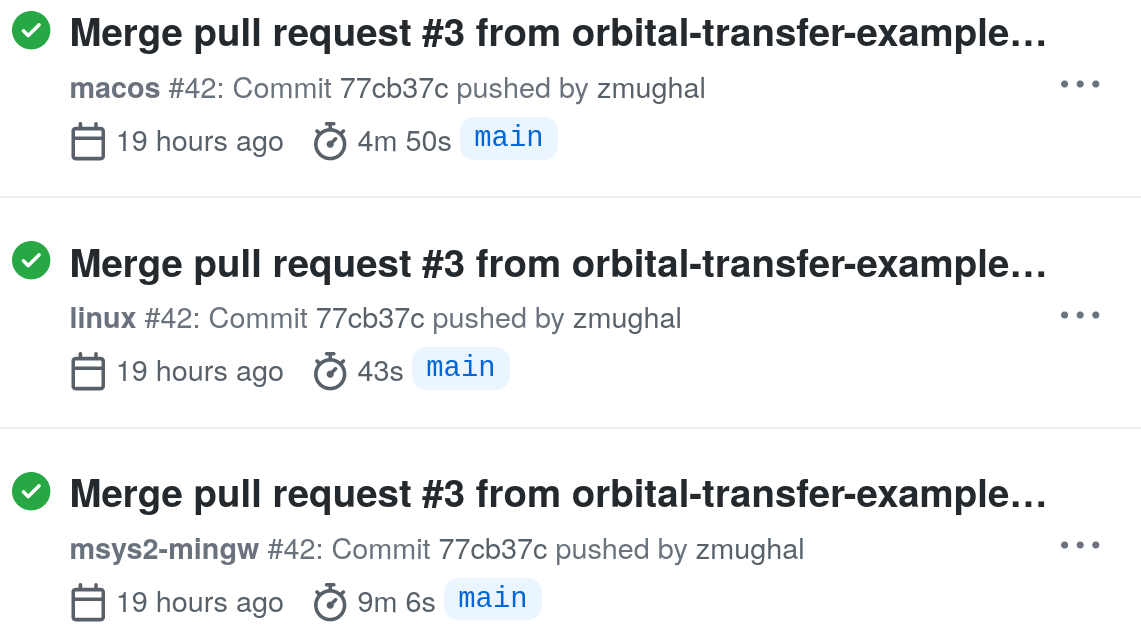
\includegraphics[height=5cm]{gfx/orbital-transfer-example-perl-gtk3-starter-basic-workflows.png}};
	\end{tikzpicture}
\end{center}
	\note{Debug build using \url{https://github.com/mxschmitt/action-tmate}}
\end{frame}

\begin{frame}[fragile]{Using Vagrant for local debugging}
Provision a VM locally
{
\setbeamercolor{block body}{bg=black}
\begin{block}{}
\begin{lstlisting}[language=sh,xleftmargin=10pt]
vagrant up buster64 # Debian
vagrant up win10    # Windows 10
#vagrant up macOS   # macOS
\end{lstlisting}
\end{block}
}
\end{frame}

\begin{frame}{Creating distributable packages}
	\begin{itemize}[<+->]
		\item Windows: \texttt{pacman -Ql}, \texttt{PAR::Packer}, WiX Toolset
		\item macOS: Homebrew tap, \href{https://github.com/create-dmg/create-dmg}{create-dmg} (\emph{TODO})
		\item Linux: .deb/.rpm, Flatpak (\emph{TODO})
	\end{itemize}
	\note{
		Example Perl Homebrew tap \url{https://github.com/sqitchers/homebrew-sqitch}
	}
\end{frame}

\section{Why I wrote a ++(document reader)}

\begin{frame}

\begin{longtable}[]{@{}c@{}}
\toprule
	\begin{minipage}[t]{0.38\columnwidth}\centering
		\href{https://doi.org/10.2200/S00215ED1V01Y200907ICR009}{Reading and Writing the Electronic Book}
		by Catherine C. Marshall
	\end{minipage}
	\tabularnewline
\midrule
\endhead
	\begin{minipage}[t]{0.38\columnwidth}\centering
		\begin{tikzpicture}
		  \node (book3) {
\includegraphics[height=3cm]{gfx/book-cover-reading-and-writing-the-electronic-book.jpg}};
		  \node (author3) at (book3.south east) {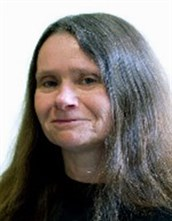
\includegraphics[height=1cm]{gfx/author-CatherineCMarshall.jpg}};
		\end{tikzpicture}
		\strut
	\end{minipage}
	\tabularnewline
\bottomrule
\end{longtable}

\end{frame}

\begin{frame}[fragile]{Curie}
\begin{center}
	\begin{tikzpicture}
	  \node (workflow) {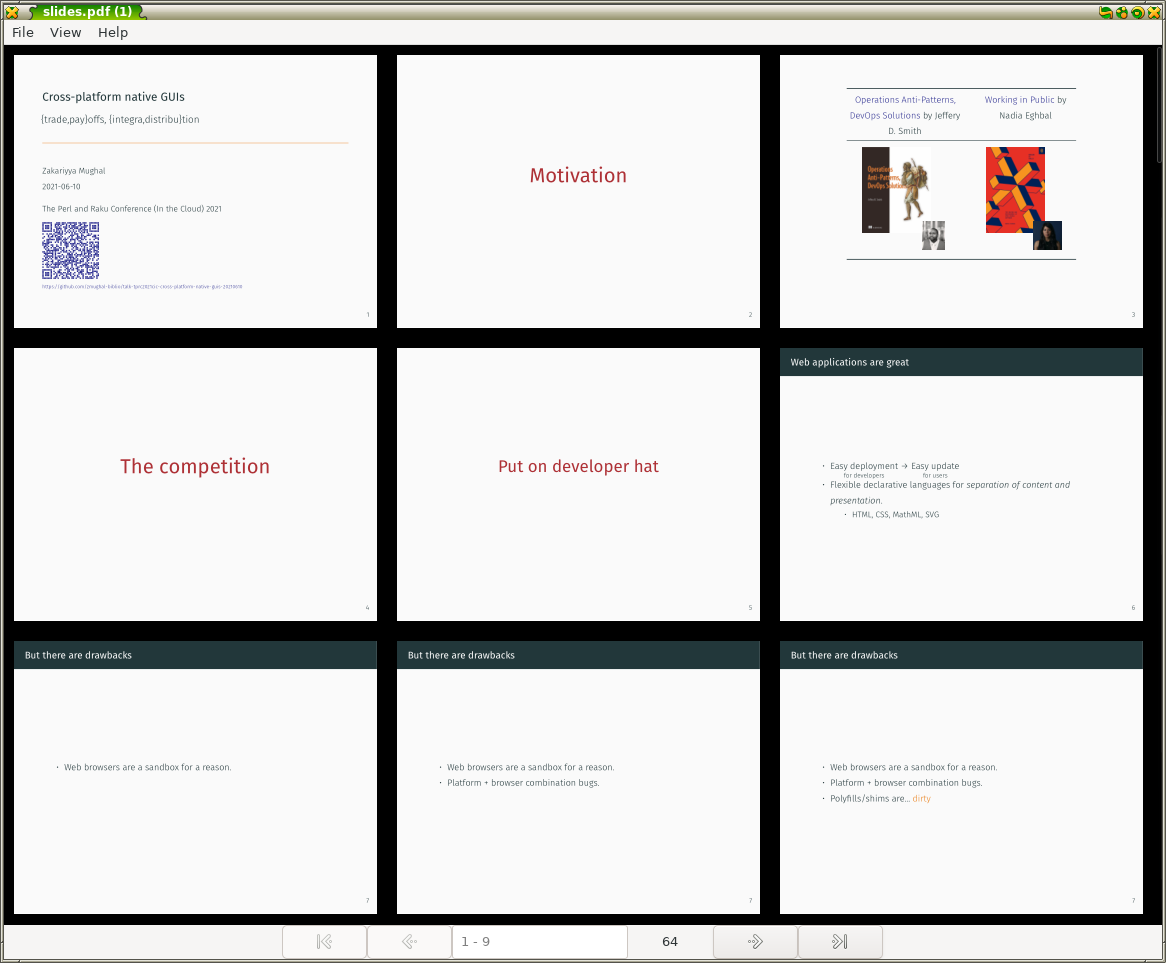
\includegraphics[height=5cm]{gfx/curie-slides.pdf.png}};
	\end{tikzpicture}
\end{center}
{
\setbeamercolor{block body}{bg=black}
\begin{block}{}
\begin{lstlisting}[language=sh,xleftmargin=10pt,escapechar=§]
cpanm -n Renard::Curie
# §\url{https://github.com/project-renard/curie}§
\end{lstlisting}
\end{block}
}

\end{frame}

\begin{frame}{Curie stack}

	\begin{multicols}{2}
	\begin{itemize}[<+->]
		\item Perl
		\item Gtk3
		\item Cairo
		\item MuPDF (Alien::MuPDF)
		\item Custom scene graph
		\item Graphene (Alien::Graphene)
		\item Kiwisolver (Alien::Kiwisolver)
		\item Festival
		\item IO::Async
	\end{itemize}
	\end{multicols}
\end{frame}

\begin{frame}{Future}
	\begin{itemize}[<+->]
		\item \href{http://androwish.org/home/home}{AndroWish}
		\item Port to e-ink device
		\item Binary Perl dist packaging on CI?
	\end{itemize}
	\note{ Compare with binary wheels in Python packaging \url{https://github.com/pypa/cibuildwheel}, \url{https://github.com/pypa/manylinux}  }
\end{frame}

\begin{frame}{Acknowledgements}
\protect\hypertarget{acknowledgements}{}

\begin{itemize}
\item
  \href{https://github.com/ChiragGhanshani}{Chirag Ghanshani},
  \href{https://github.com/svyotov}{Stanislav Yotov},
  \href{https://twitter.com/j3sus_h}{Jesus Hernandez}
\item
  \href{https://github.com/cpan-testers/cpantesters-project}{CPAN
  Testers}, \href{https://metacpan.org/author/SREZIC}{Slaven Rezić},
  \href{https://metacpan.org/author/CONTRA}{Thibault Duponchelle}
\item
  \href{https://github.com/PerlAlien}{PerlAlien},
  \href{irc://irc.perl.org/\#native}{\#native},
  \href{https://mail.gnome.org/archives/gtk-perl-list/}{GTK-Perl mailing list}
\end{itemize}

\end{frame}

\begin{frame}{Questions \& Contact} % Questions
\begin{itemize}
	\item on IRC: \texttt{sivoais} on \url{irc://irc.perl.org/\#native}
		(Alien and FFI!) or \url{irc://irc.perl.org/\#pdl} (scientific and numerical computing!),
	\item on Twitter: \href{https://twitter.com/zmughal}{@zmughal},
	\item on GitHub: \url{https://github.com/zmughal}.
\end{itemize}

\end{frame}

\end{document}
